\chapter{Data Reductions}\label{chap:introduction}

In this chapter, we will discuss the Astronomical codes/programs that we employed in our study. After obtaining these high-resolution spectroscopy observations, for thirteen stars, we had to reduce these observational data and turn them into normalized 1D spectra. We achieved our goal by using the Image Reduction and Analysis Facility \citep[][hereafter IRAF]{1986SPIE..627..733T, 1993ASPC...52..173T} and its packages.


\section{Data reductions with IRAF}
This section aims to obtain a wavelength-calibrated spectrum from the two dimensional CCD image; calibrations of CCD data, extraction of the spectrum, wavelength calibration, continuum normalization, and combining spectra of individual echelle orders. Figure \ref{chart} shows a chart-flow for the echelle reduction procedure.

\vspace{5mm}
\begin{figure}[!ht]
\centering
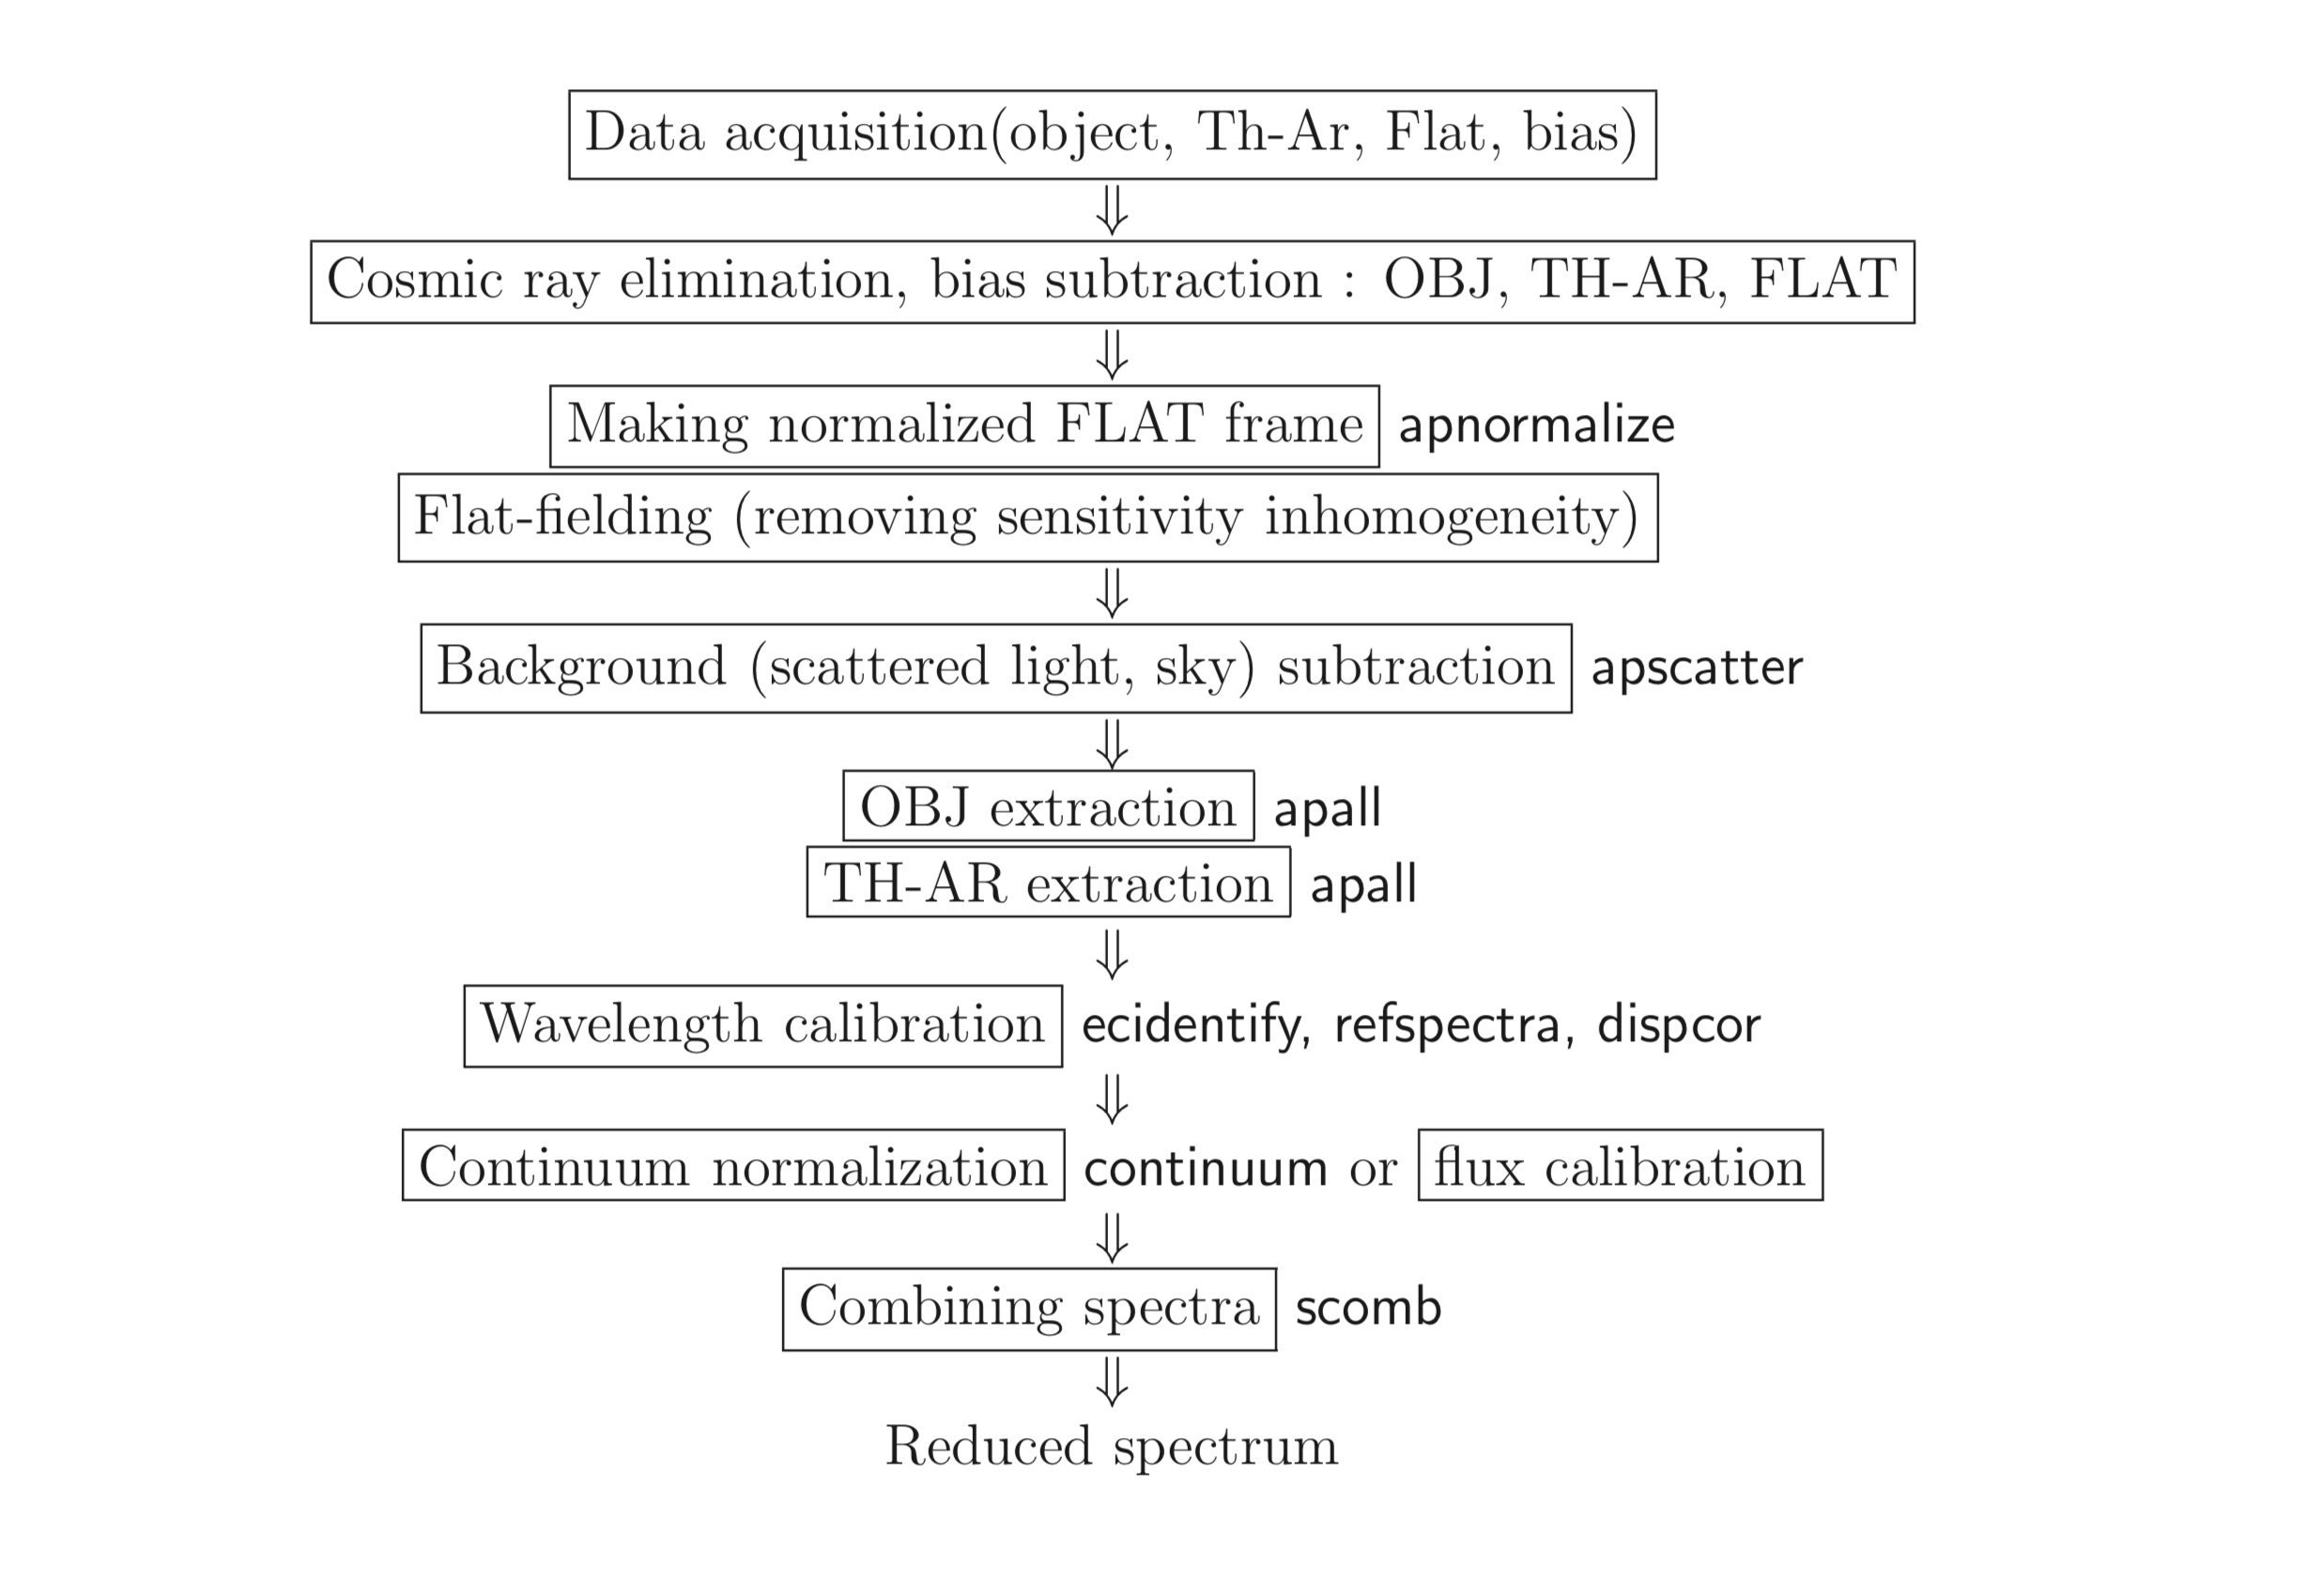
\includegraphics[width=\textwidth, angle=0]{Img/flow-chart.png}
\caption{Chart-flow for the echelle reduction procedure.} 
\label{chart}
\end{figure}

\newpage

\begin{description}
\item[Dark currents and Bais corrections:] \hfill \\ The first step in our data reduction was the bias\footnote{The Bias can be estimated by obtaining some CCD values with no exposure time (zero seconds); } and dark current\footnote{Dark currents determined without opening the CCD shutter.} corrections. To improve the data quality we combined several Bias files by using the average Bias value of every pixel; in case of cosmic-ray noise, some pixels will show high Bias values, which makes the statistical median is the right choice rather than average.
  
\item[Extraction of spectra:] \hfill \\ The second step in our data reduction was extraction of spectra. It is useful to generate a reference frame for the consequence steps using the apall task. The second step in our data reduction was extraction of spectra. It is useful to generate a reference frame for the consequence steps using the apall task, which examines the individual echelle orders for spectra and then estimate the aperture's position and size. Moreover, this step can be interactively corrected (see top right panel of Figure \ref{reductions})

\item[Flat fielding:] \hfill \\ The third step in our data reduction was the flat fielding. In this step, we did a pixel-to-pixel correction to remove any sensitivity inhomogeneity of the CDD. At the time that a wavelength coverage of the spectrograph is so broad (as the case in the APF data), the flat lamp intensity/strength might not be adequately high in some ranges. Therefore, we alter the exposure time of the flat data, either the filter setting. The APF data has narrow and wide flat data for each CCD. We normalized all the flat frames and then divided the science object frame by the new combined flat frame.

\item[Background subtraction:] \hfill \\ The third step in our data reduction was the background subtraction. The IRAF apscatter task did this step. This step can be interactively corrected (see top left panel of Figure \ref{reductions}). One might alter the fitting function either its order. Once the fitting seems satisfactory, we proceed with the remaining steps.

\item[Extraction of one dimensional spectra:] \hfill \\ The fourth step in our data reduction was extraction of one dimensional spectra. We had used the task apall one more time to extract the spectrum from the object frame, which we previously flat-fielded and background-subtracted.

\item[Wavelength calibration:] \hfill \\ The fifth step in our data reduction was the wavelength calibration. In this step, we linked comparison data, previously mentioned, to produce wavelength scale using refspectra task. Figure \ref{reductions}, lower right panel shows the result of this step.

\item[Continuum normalization:] \hfill \\ The sixth step in our data reduction was the continuum normalization. In this step, we obtained normalized spectra by fitting curves. The efficiency of the APF Echelle spectra is somewhat near the CCD center. Moreover, the edges show deficiency at spectra ends/edges. We altered the fitting function and its order until the fitting is pleasing. The exercise wa done for all apertures/orders. Figure \ref{reductions}, lower left panel shows the result of this step.

\item[Doppler effect:] \hfill \\ The final step, in our data reduction, was doppler correction. In this step, we prepare our normalized spectra for the chemical abundances' investigation. We shifted our normalized spectra to its rest frame, using FXCOR task. Finally, we used wspectxt task to write the RV corrected spectra into an ASCII file (two columns; wavelength and normalized flux).

\end{description}







\begin{figure}[t!]
{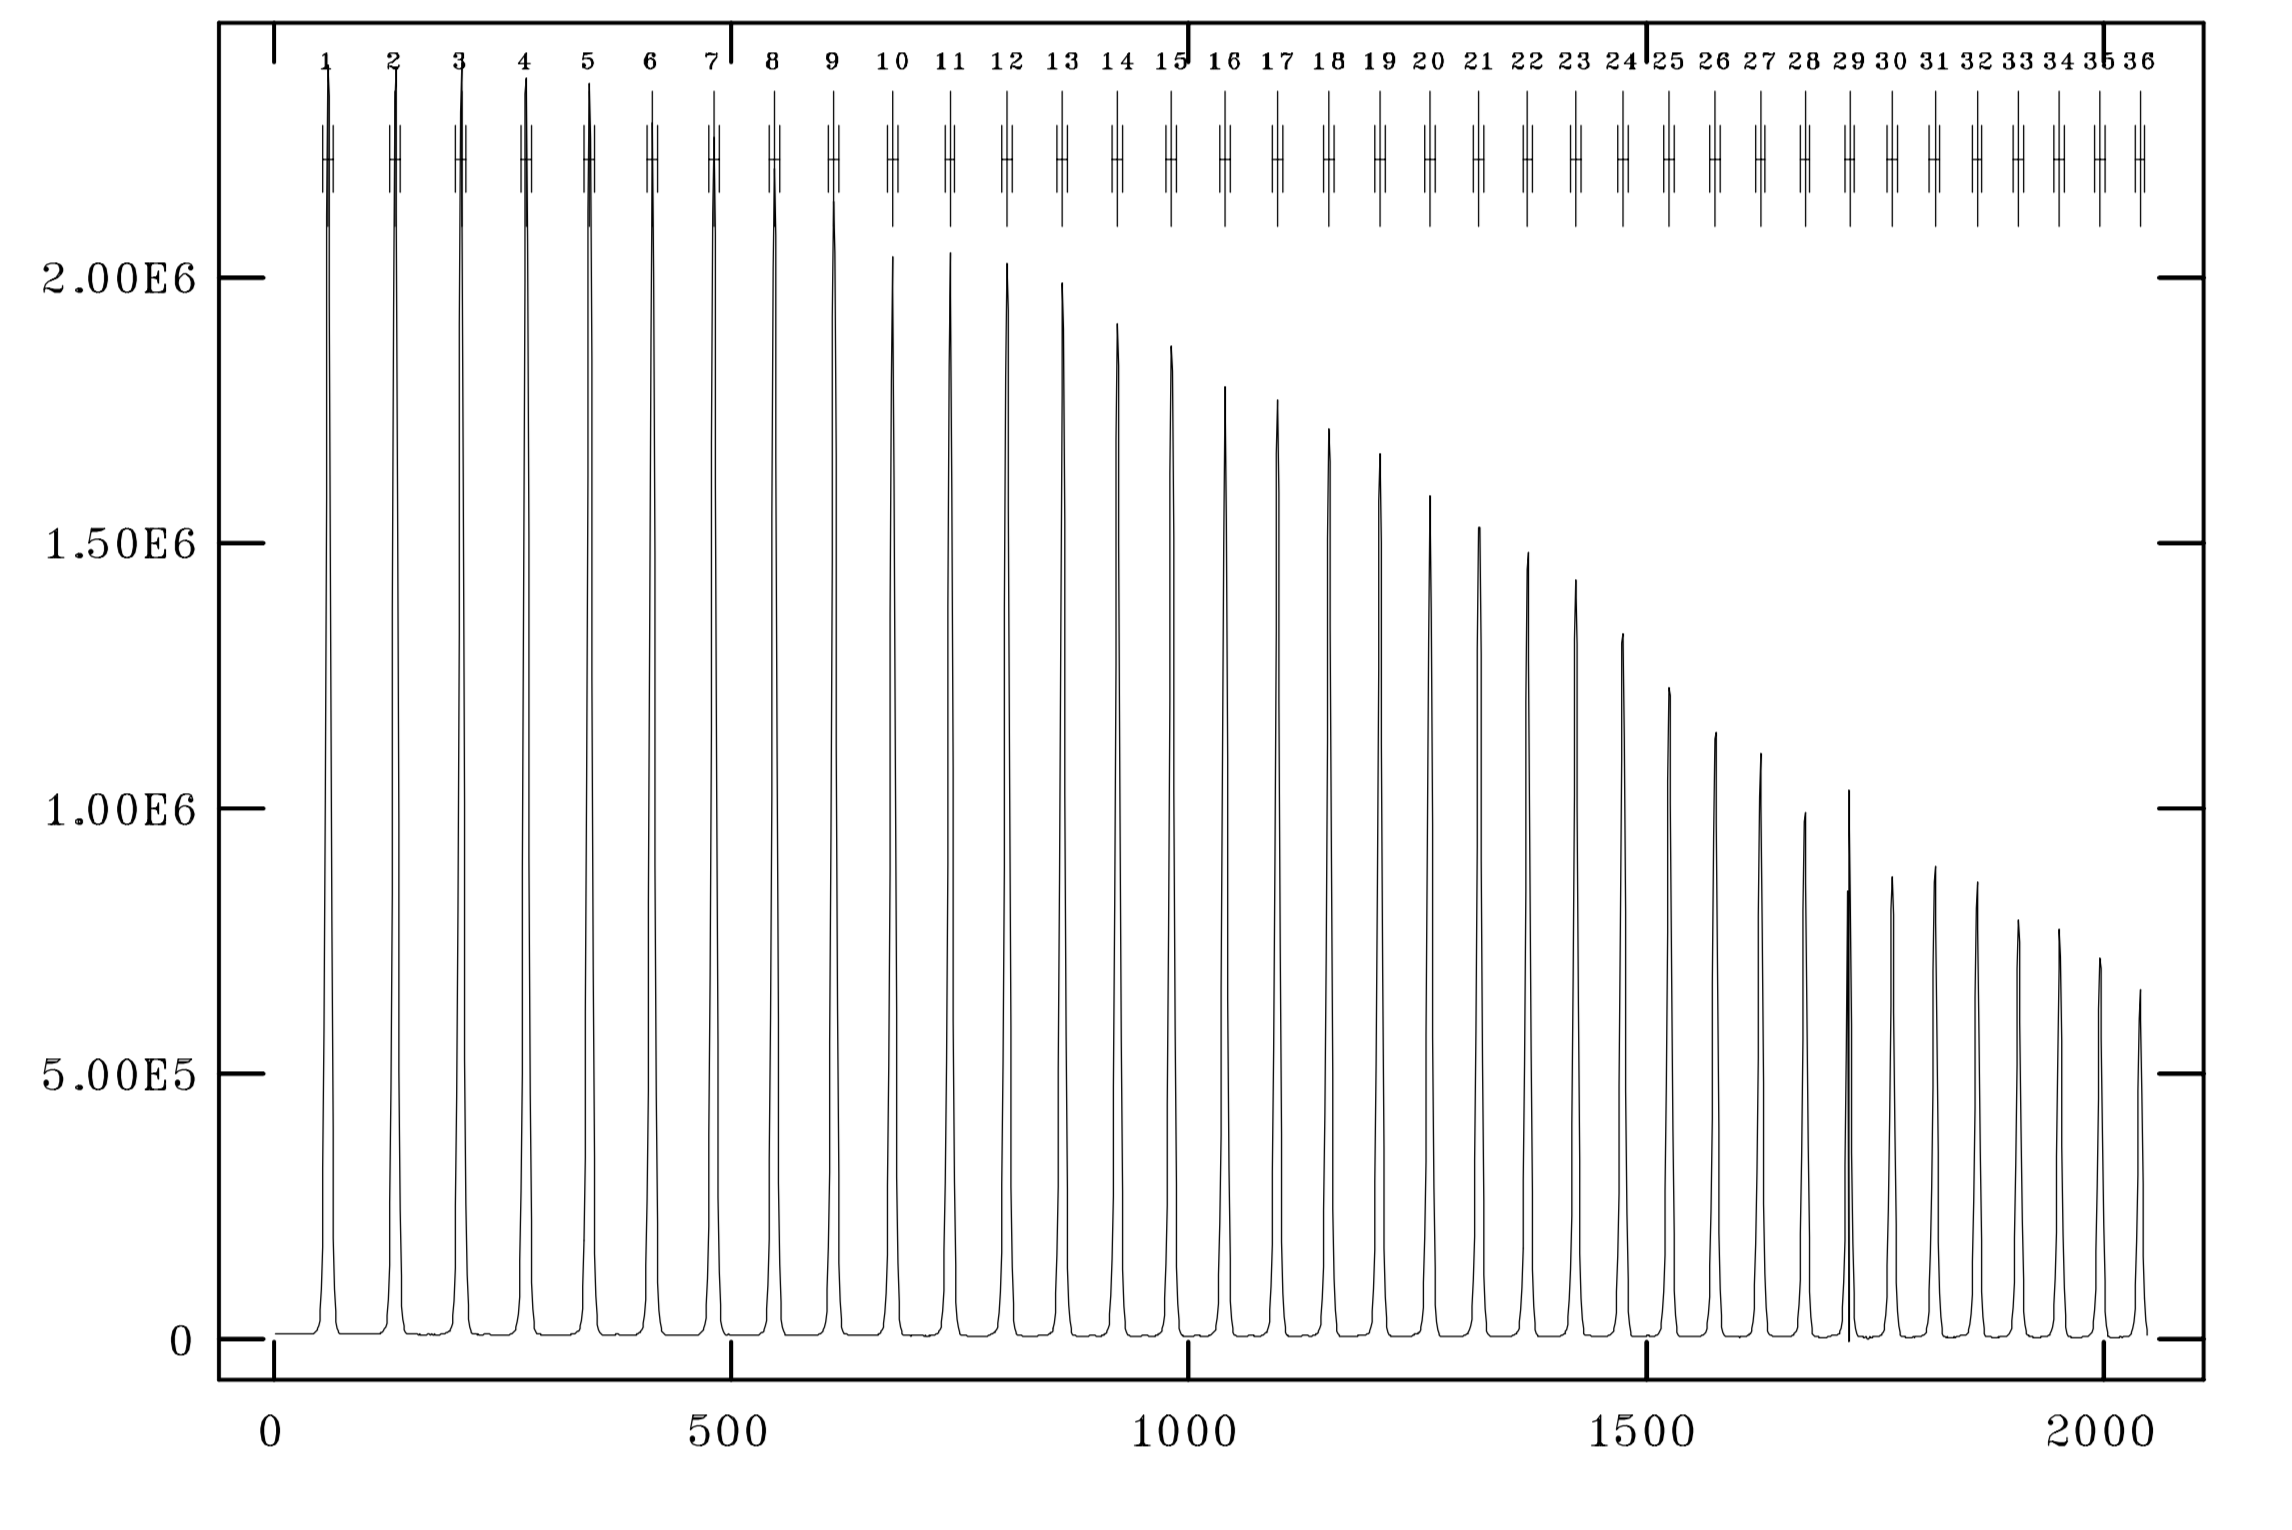
\includegraphics[width = 0.55\textwidth]{Img/Extraction_of_spectra.png}}
{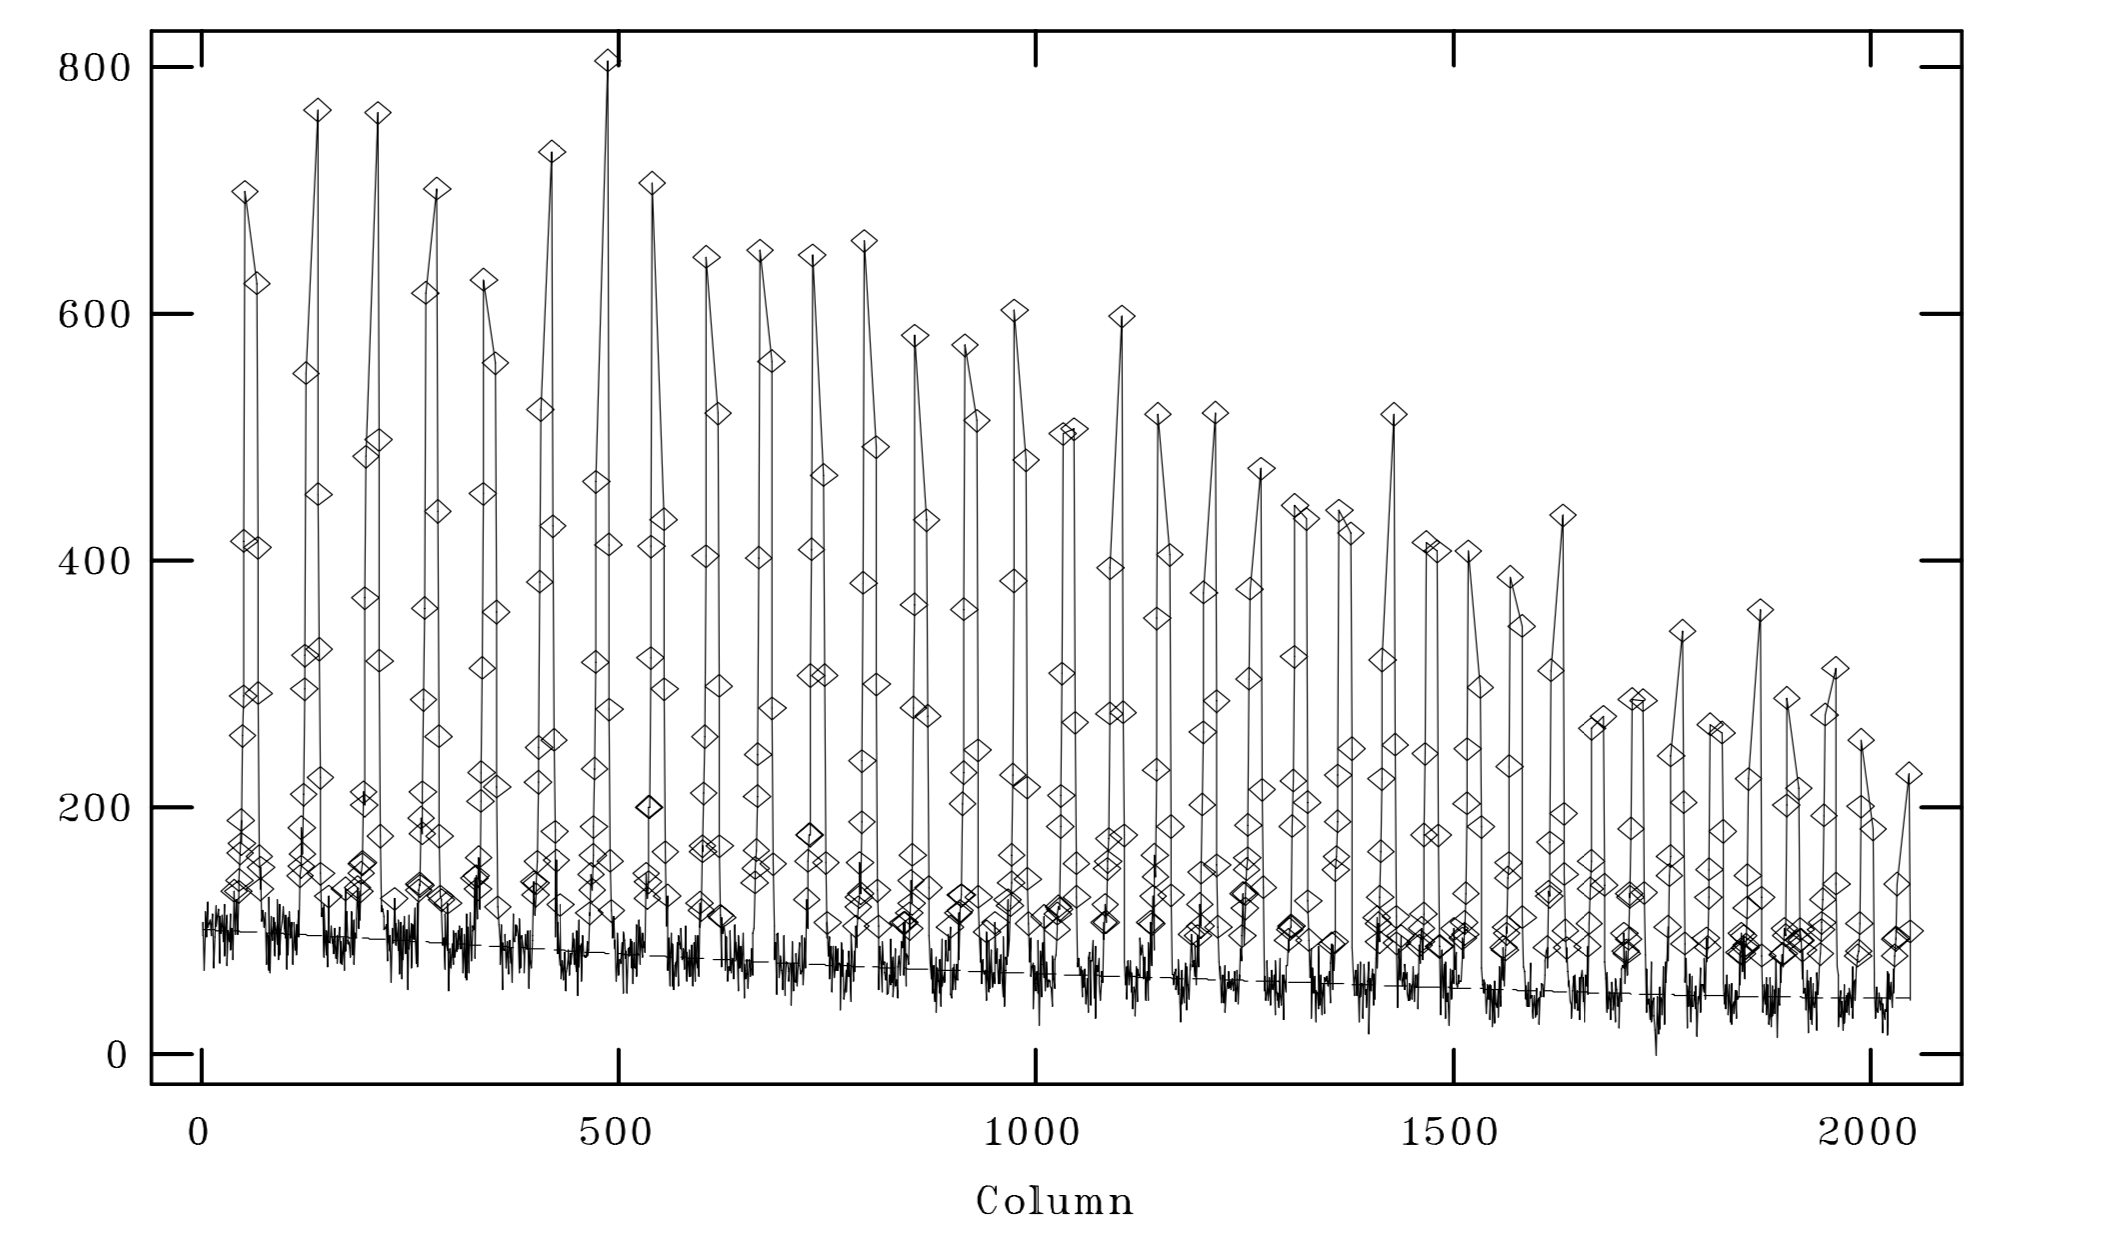
\includegraphics[width = 0.55\textwidth]{Img/Background_subtraction.png}}\\
{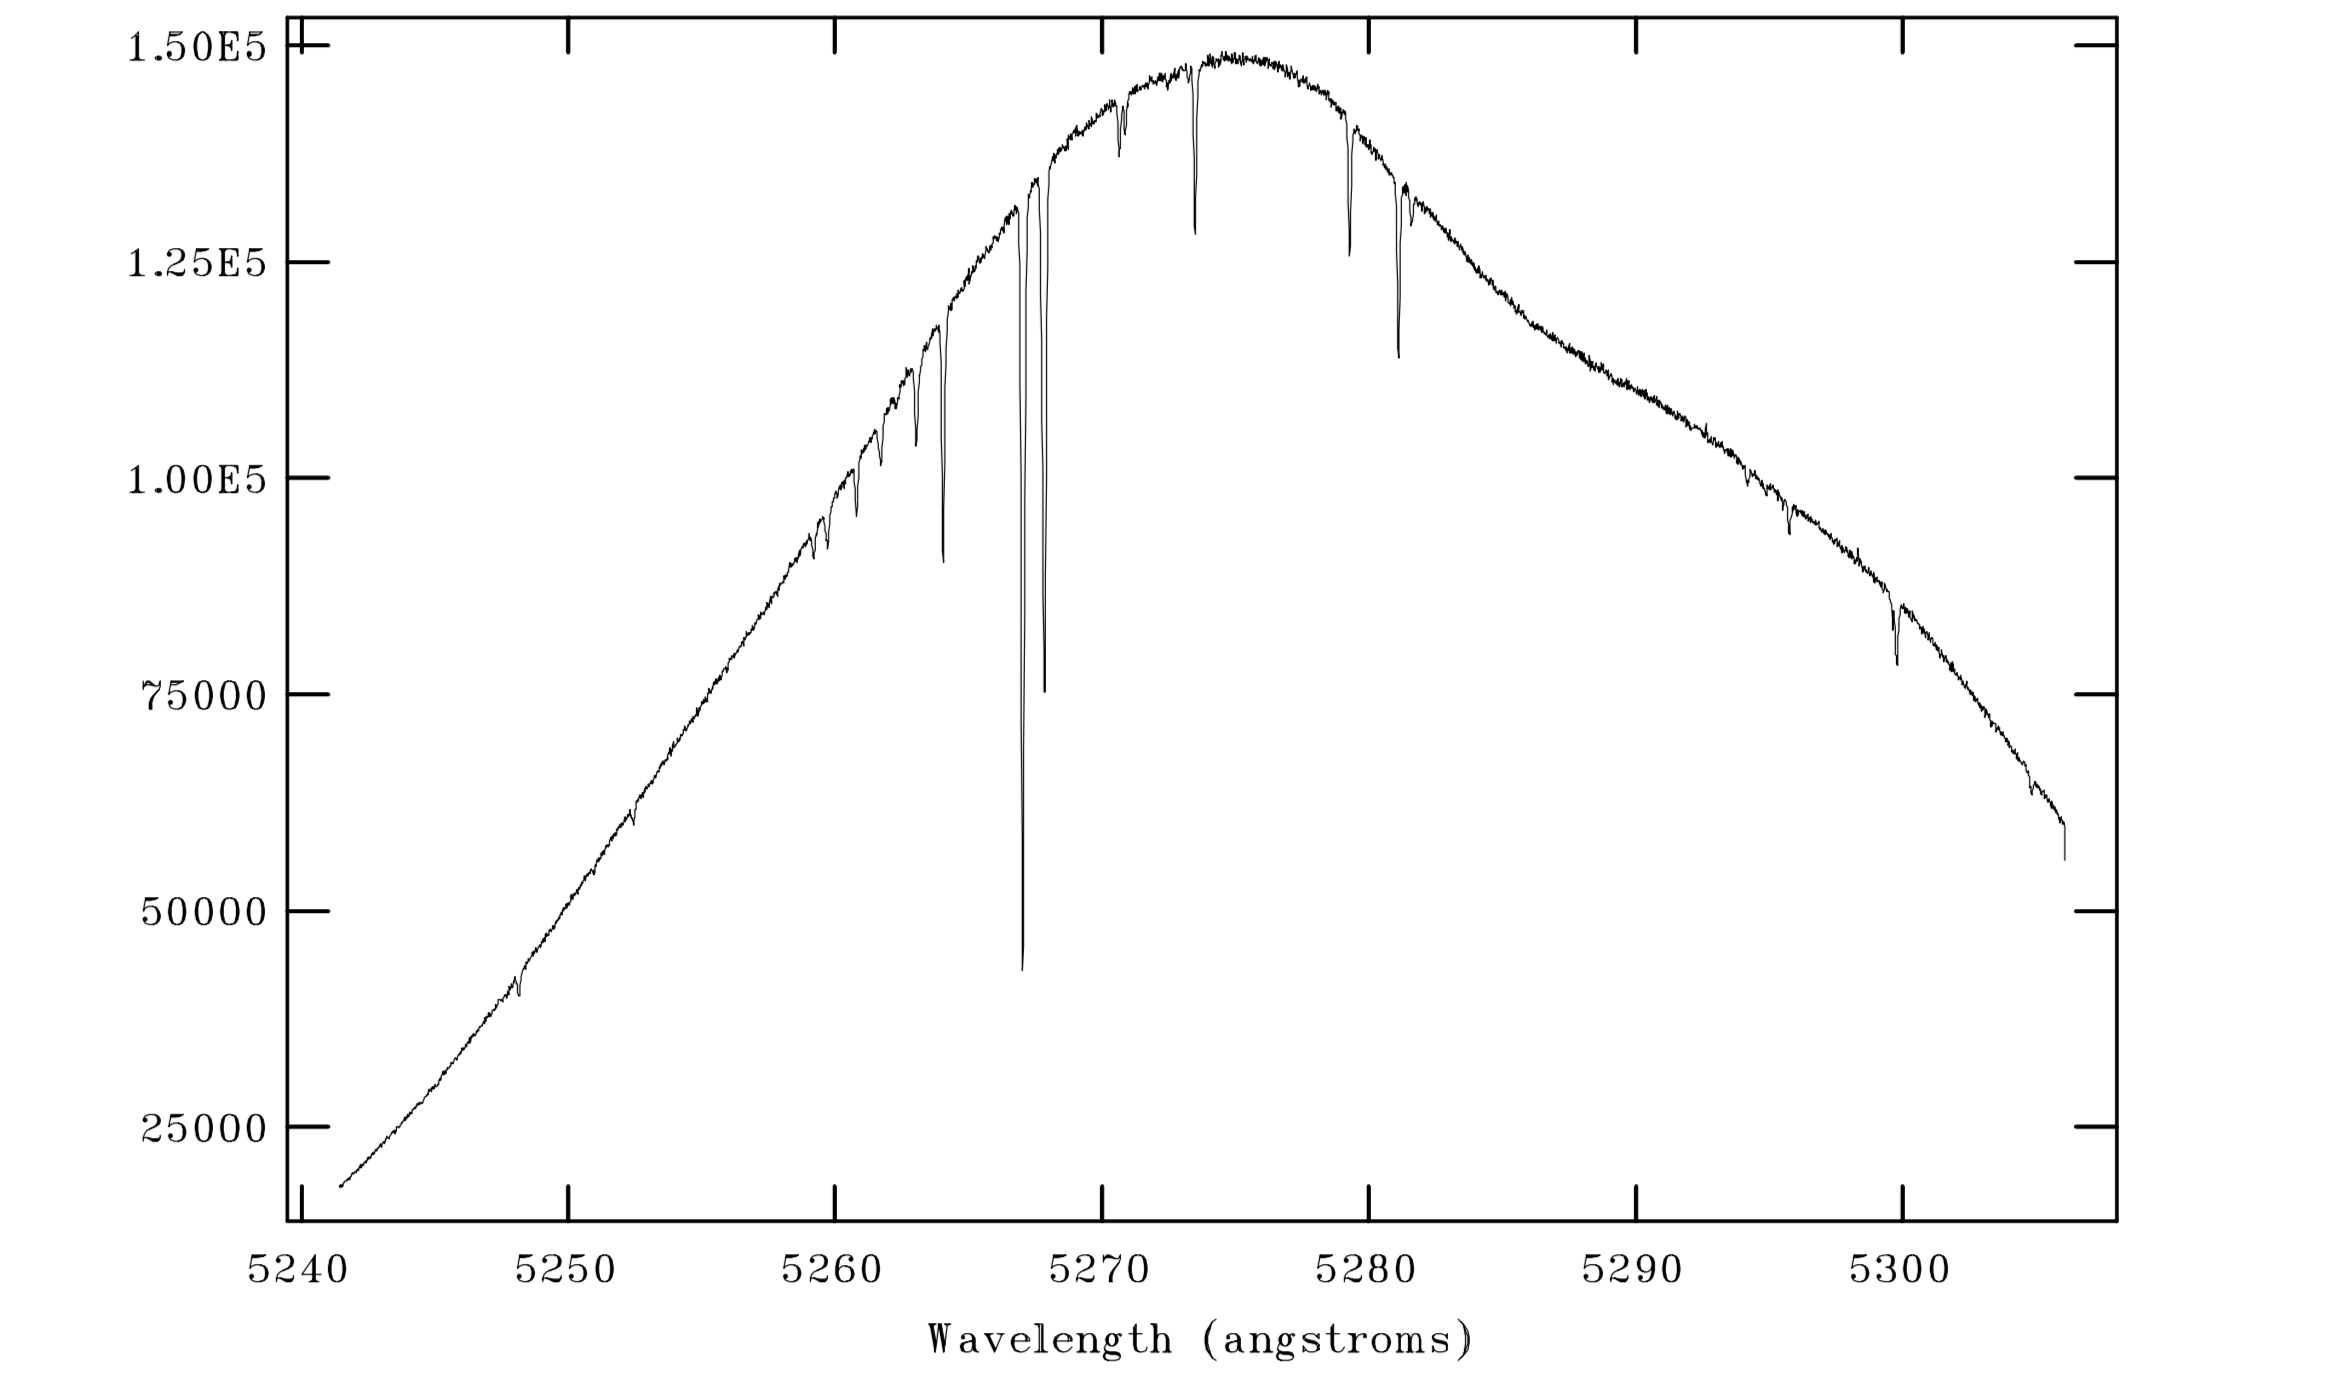
\includegraphics[width = 0.55\textwidth]{Thesis/Img/wavelenght.png}} 
{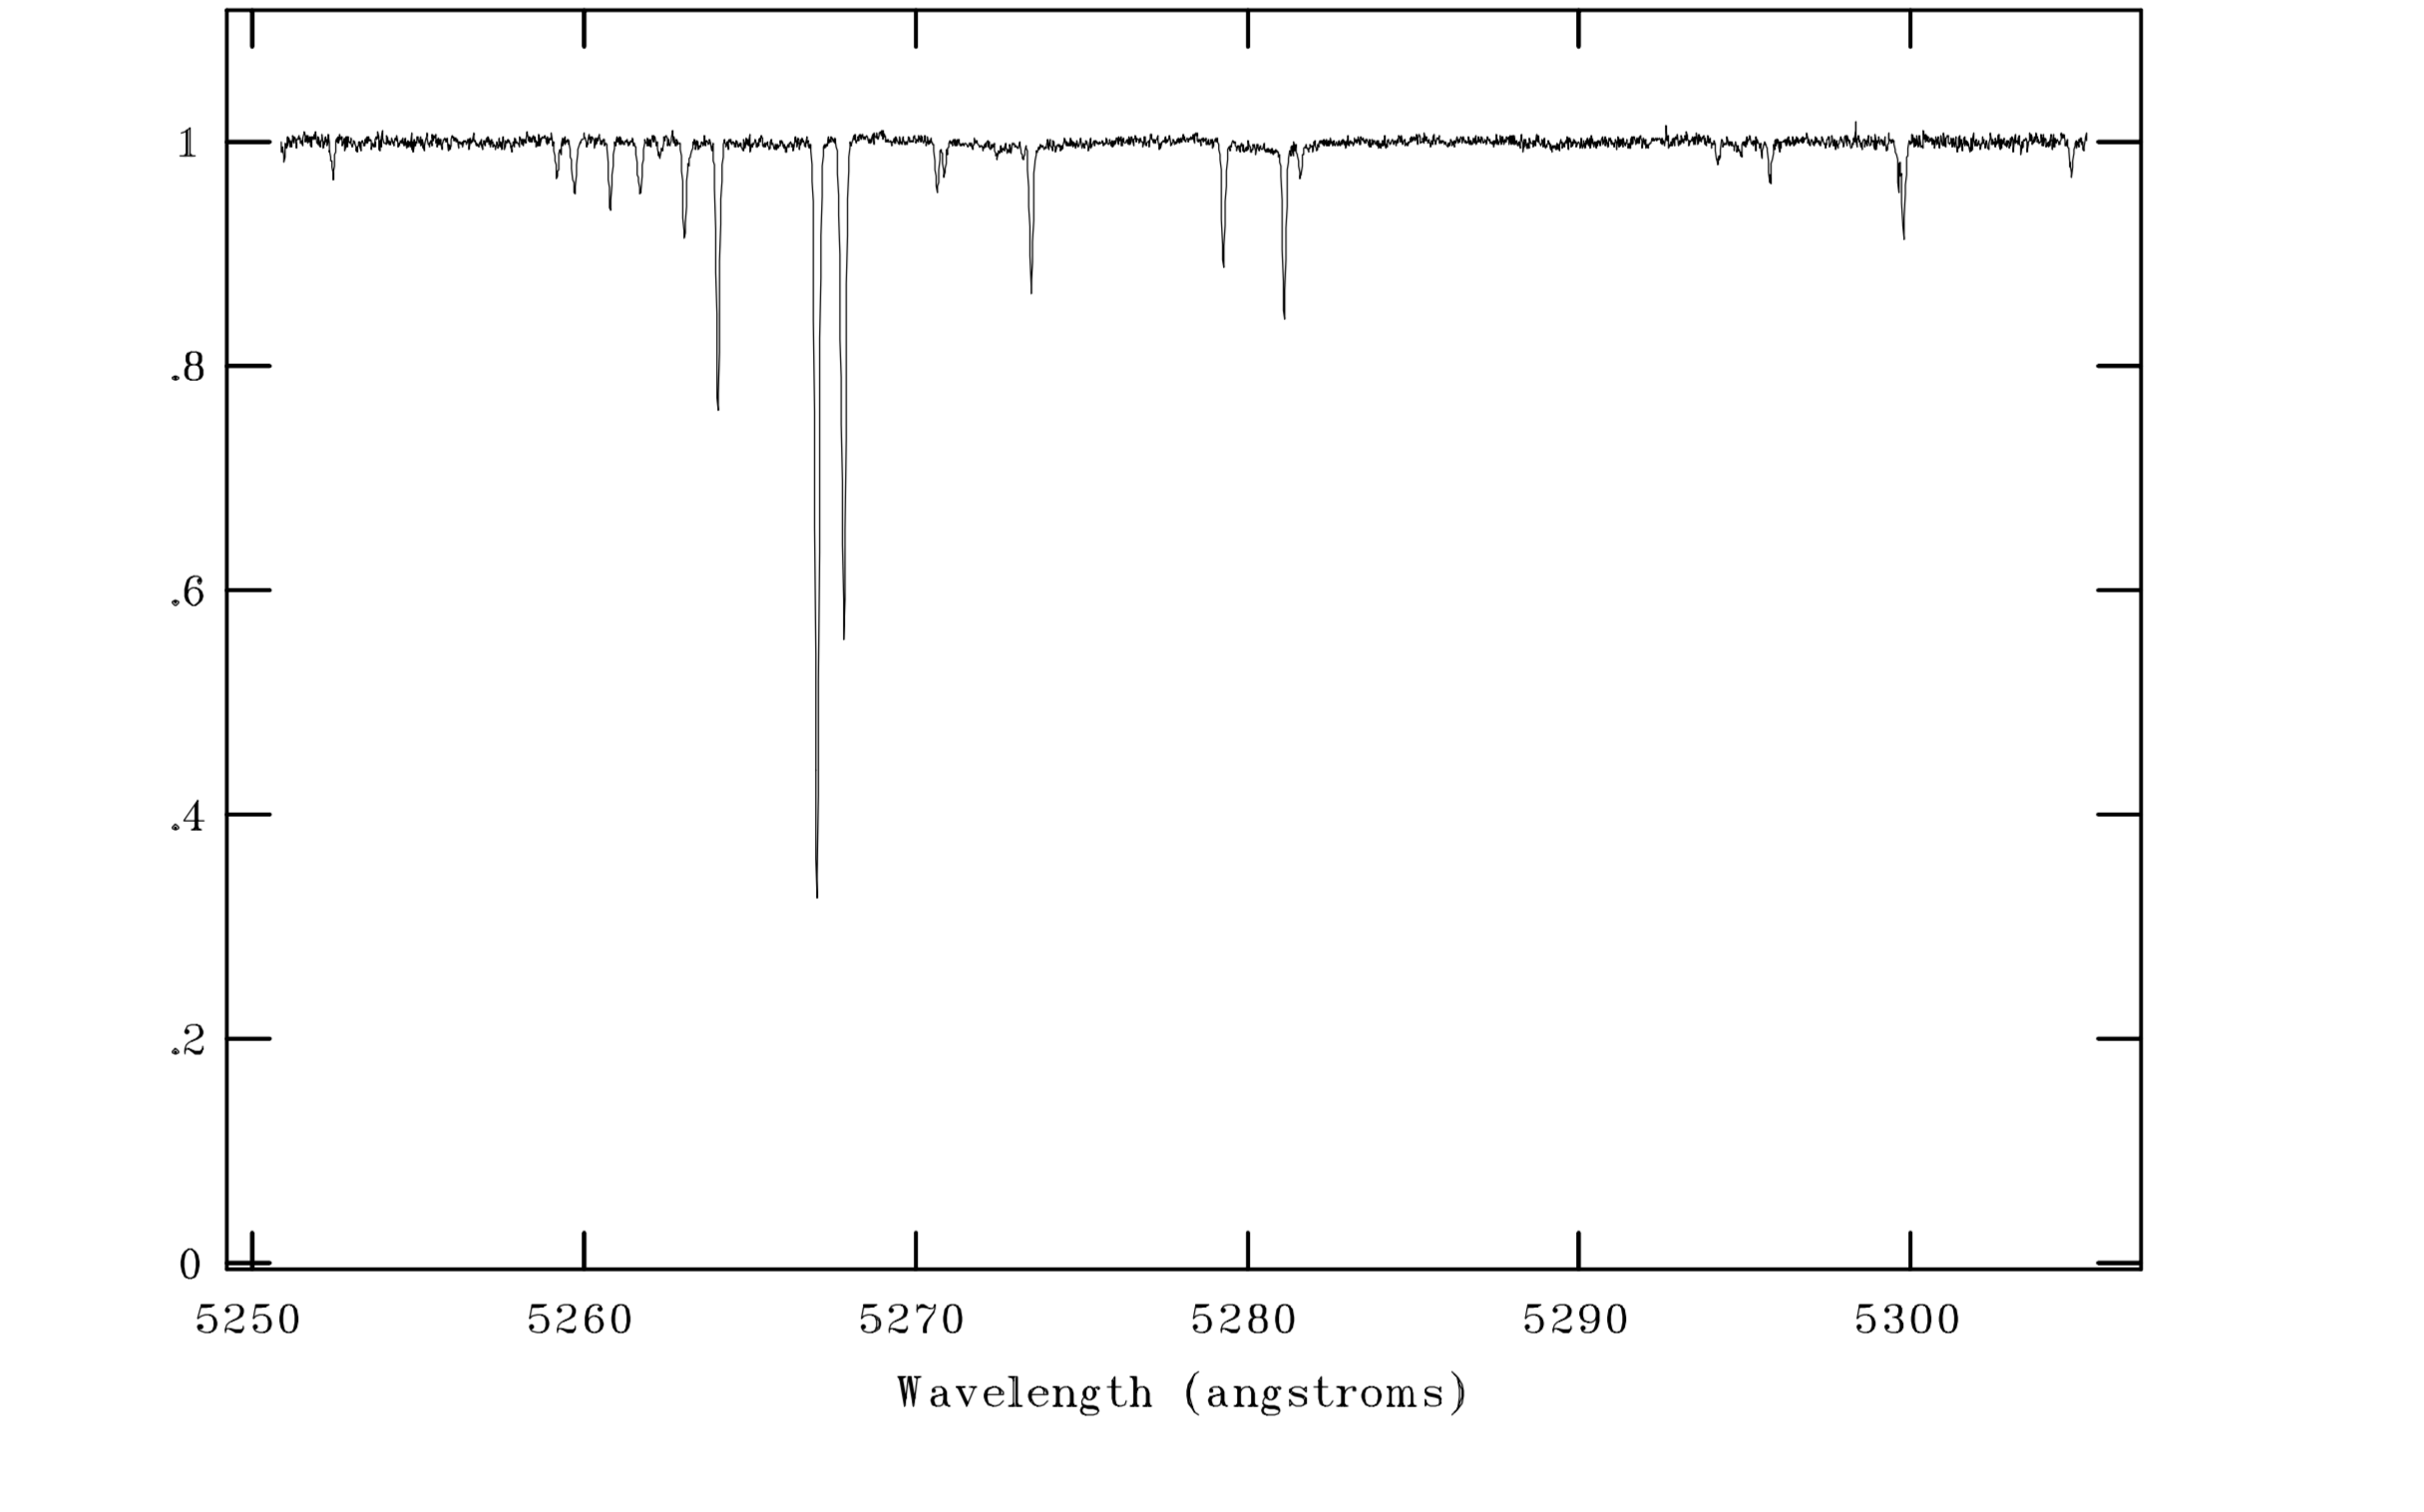
\includegraphics[width = 0.55\textwidth]{Thesis/Img/normalized.png}}\\
\caption{An illustrative example of our data reduction procedures for the major steps.}
\label{reductions}
\end{figure}



